\Chapter{Tesztelés}

\Section{Felhasználói kézikönyv}

Ahhoz hogy az AI ellen tudjunk játszani, először telepítenünk kell az OpenTTD-t. Ha ez megtörtént, az AI fájljait a játék mappájában lévő "\textit{ai}" nevű mappába kell bemásolnunk. Ennek az útvonala alapértelmezett telepítési beállítások mellett Windows-on "\texttt{C:\textbackslash Program Files\textbackslash OpenTTD\textbackslash ai}". Miután bemásoltuk az AI mappáját a játékéba, az elindítást követően az "MI/Játékszkript beállítások" menüpontban van lehetőség gépi ellenfél hozzáadására, az ilyenkor megnyíló helyre be lehet állítani a DebacleAI-t mint ellenfél. Ezt követően egy új játék megkezdésekor az AI automatikusan el fog indulni.

Ezek után egyéb figyelmet az AI nem igényel, a felhasználó szabadon játszhat a játékkal, miközben az AI is a korábban bemutatott módon fogja játszani a játékot mint egy rivális cég a pályánkon.

Abban az esetben ha az AI futás idejű problémába ütközne, a játék értesíteni fogja erről a felhasználót. Ebben az esetben a nyomkövetés ablakában lévő MI újratöltése gombbal van lehetőségünk újraindítani az AI-t. Ennek az ablaknak magától is meg kellene nyílnia, de abban az esetben ha ez nem történne meg, a felső eszközsáv utolsó gombját (kérdőjel egy kék körben) lenyomva tartja tudjuk elérni az "MI/Játékszkript nyomkövetés" pontban.

\Section{Megfigyelések}

Már a rövid fejlesztési folyamat közben is észrevehető volt, hogy az AI képes a játékmenet fenntartására, és nyereség generálására is, tehát ebből a szempontból a saját stratégia megvalósítása sikeresnek nevezhető. Ugyanakkor, az AI csak utasok szállításával foglalkozik buszok segítségével, a többi szállítási lehetőség egyáltalán nincs lefedve az AI által.

Ezzel szemben más AI-oknak sokkal kifejlettebbek. Az általános AI-ok minden szállítási lehetőséggel, és sokkal stabilabban futnak, kevesebb hibába ütköznek és több profitot is képesek generálni. Ez annak is betudható, hogy a legtöbb AI éveken keresztül haladt át a fejlesztési folyamaton és ennél még hosszabb tesztelési fázison. Ami közben és után, elérhető volt a BaNaNaS repository részeként, így játékosok százai tudták kipróbálni őket, és visszajelzést adni adott hibákról, problémákról vagy ötletekkel hozzájárulni a folyamathoz. A fórumbejegyzéseket olvasva megállapítható, hogy a problémák többsége ami felléphet a játék folyamán a következőek: 

\begin{itemize}
	\item Útvonal/hálózat tervezéssel kapcsolatos problémák
	\item Útvonalkereső hatékonyságához köthető hibák
	\item Adott út/vasúthálózatok túlterhelése járművekkel
	\item Pénzügyi problémákkal kapcsolatos észrevételek
	\item Létező infrastruktúra újrahasznosításával kapcsolatos problémák
\end{itemize}

Ebből a lényeges információ amire következtethetünk, hogy függetlenül a fejlesztési időtől vagy a tesztelők számától, még a legrégebbi és legátfogóbb AI-okban is jelentkezhetnek problémák. Ezeket a megszokott módon a fórumbejegyzésekben szokták megtenni, megfigyelhető, hogy 10 évvel ezelőtt fejlesztett AI-ok bejegyzéseiben még a tavalyi év folyamán is érkeztek bejelentések hibákról. Tekintve, hogy a játék környezete nagyon dinamikus, és az AI megvalósításának problémája mennyire komplex, nehéz teljesen ideális, vagy hibátlan állapotot elérni.

Ahogyan \aref{fig:atlag} ábrán megfigyelhető, egy átlagos futtatási szituációban az AI jó eredményeket képes produkálni. Itt látható, hogy a 10 éves folyamat alatt:

\begin{itemize}
	\item 152 jármű zárta profittal az előző évet,
	\item A közelmúltban 67 állomást szolgált ki,
	\item Az előző negyedév profitja 74 százalékkal nagyobb az elmúlt 12 negyedév maximális profitjánál,
	\item 22.147 utast szállítottunk el ez előző negyedévben,
	\item Az felvett kölcsön mennyisége 0.
\end{itemize}

\begin{figure}
	\centering
	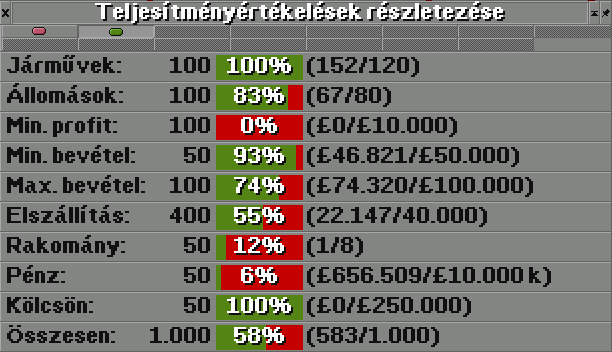
\includegraphics[scale=0.7]{images/atlag.png}
	\caption{A DebacleAI kiértékelése egy 10 éves játékfolyamat után.}
	\label{fig:atlag}
\end{figure}

\Section{Tesztelési körülmények}

A következő részekben az AI-ok teljesítményének az összehasonlítását fogom bemutatni. Ehhez az AI-okat egy játékkörnyezetben futtattam 10 évig. Ezekben a játékokban, a pályagenerálás beállításai mindig ugyan azok voltak. Ezek pedig az alábbiak:

\begin{itemize}
	\item Térkép mérete: 256x256
	\item Térkép generátor: TerraGenesis
	\item Várossűrűség: Normál
	\item Gazdasági épületek száma: Normál
	\item Tereptípus: Sík
	\item Tengerszint: Nagyon alacsony
	\item Simaság: Sima
	\item Folyók: Közepes
	\item Dátum: 1950 Jan. 1.
	\item A térkép határa minden esetben víz
\end{itemize}

Az olyan AI-ok esetében, ahol a megvalósítás általános, és többféle szállítási módszert is tudnak használni, a működést lekorlátoztam buszok használatára. (A SimpleAI esetében erre nem volt lehetőség, azt csak közúti járművekre lehet korlátozni) Ennek az volt az oka, hogy összehasonlítás szempontjából, az olyan AI-okkal szemben amelyek csak utasokat szállítanak, vagy csak közúti járműveket használnak, sokkal nagyobb bevétel generálására lettek volna képesek a piaci rés kihasználásával.

\Section{Önálló tesztelés}

